\chapter{Magnetic field simulation in ND280}
\label{chap:MagneticFieldSimulation}
ND280 is housed in the \Yoshi{former}{it isn't the UA1 magnet any more!} UA1 magnet which provides a \Yoshi{0.18}{It's not a 0.2 T field any more!}~T magnetic field through the basket.  The purpose of this magnetic field is to aid particle \Yoshi{identification}{was identifcation} \Yoshi{and momentum measurement}{not just PID} in ND280's TPCs.  This magnetic field is accurately modelled in nd80mc by a constant 0.2 T magnetic field in the basket.  The ND280 analyses, which are inputs to the oscillation analyses, search for a TPC track matched to an FGD track so, in a first iteration of these analyses, the magnetic field model is sufficient for its purpose.
\newline
\newline
However, a significant part of the UA1 magnet is the iron based, magnetic flux return yoke which helps to tightly contain the magnetic field outside of the tracker region.  As a result, there is a significant magnetic field contained within the magnetic flux return yoke during operation.  This magnetic field in the flux return yoke is not modelled in nd280mc.  For the first iterations of the ND280 oscillation input analyses, this approximation was valid.  However, as the ND280 analyses become more mature, and non-tracker based analyses are started, this approximation is no longer sufficient.  So, the magnetic field model in the simulation needs revising.

\Yoshi{As a core feature of the presented analysis requires}{I would add something like ``As one of the analysers who has been central to studying events occurring in the ECals, which are directly affected by mismodelling of the magnetic field in the yokes, I was the first T2K collaborator to investigate this effect and provide an improved field model; this was subsequently adopted as the field to be used in official ND280 MC simulations, used by all physics analyses at ND280.}

\section{Magnetic field model in the ND280 flux return}
\label{sec:MagneticFieldModel}
\begin{figure}
  \centering
  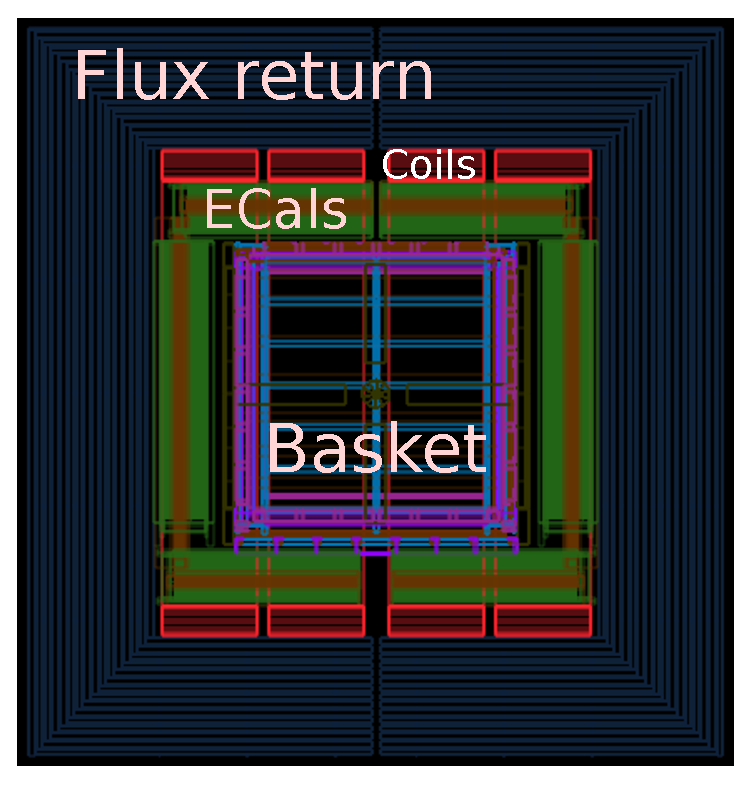
\includegraphics[width=9cm]{images/magnetic_field/ND280FluxReturn}
  \caption{Graphical display of the X-Y ND280 cross-section.}
  \label{fig:ND280FluxReturn}
\end{figure}
A simple model for the magnetic field in the flux return can be found by making two assumptions.  Firstly, the flux return yoke consists mostly of iron which has a much higher magnetic permeability than the air surrounding it.  So, it can be assumed that any magnetic flux passing through the ND280 basket is solely transported back around by the return yoke (no flux passes through the atmosphere in the pit).  It follows that
\begin{equation}
  \phi_{\textrm{b}} = \phi_{\textrm{r}},
  \label{eqn:BFluxConservation}
\end{equation}
where $\phi_{\textrm{b}}$ is the magnetic flux passing through the tracker and $\phi_{\textrm{r}}$ is the magnetic flux passing through the return yoke.  The second assumption regards the shape of the ND280 basket and flux return yoke.  The X-Y cross-section of ND280, as shown in Fig.~\ref{fig:ND280FluxReturn}, can be modelled as two distinct parts: the flux return yoke and everything contained within.  It is clear from Fig.~\ref{fig:ND280FluxReturn} that both areas are \Yoshi{rectangular}{retangular} so the system can be modelled as a smaller rectangle (the basket) contained within a larger rectangle (the return yoke).  Using this assumption and Eq.~\ref{eqn:BFluxConservation}, the magnetic field strength passing through the return yoke, $B_{r}$, is
\begin{equation}
  B_{\textrm{r}} = \frac{B_{\textrm{b}}A_{\textrm{b}}}{A_{\textrm{r}} - A_{\textrm{b}}},
  \label{eqn:FluxReturnBField}
\end{equation}
where $B_{\textrm{b}}$ is the strength of the magnetic field passing through the basket, $A_{\textrm{b}}$ is the cross-sectional area of the basket region and $A_{\textrm{r}}$ is the cross-sectional area of the flux return yoke if the flux return yoke was not hollow.
\newline
\newline
\begin{figure}
  \centering
  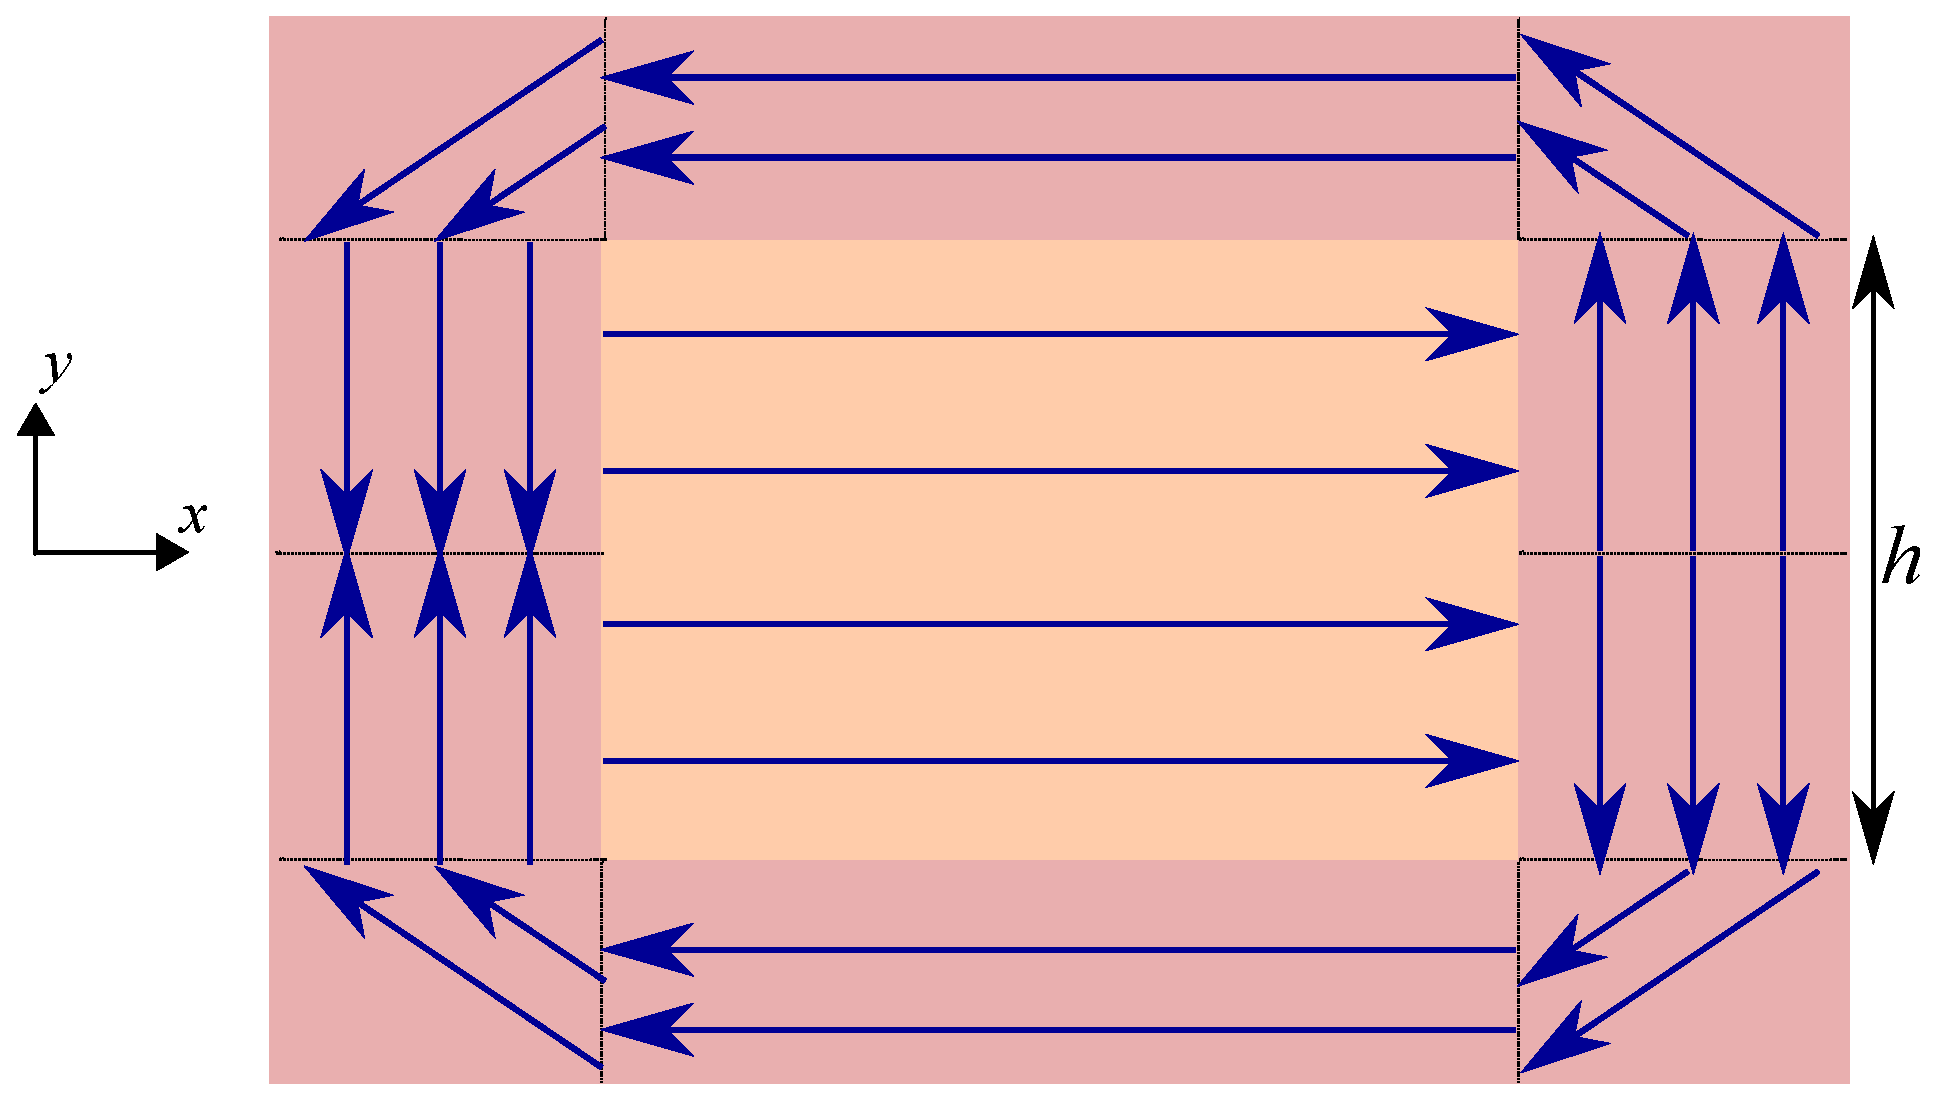
\includegraphics[width=9cm]{images/magnetic_field/BFieldDiagram}
  \caption{Simple model of the magnetic field in the basket and flux return region.  The flux return yoke has been separated into ten sections: four vertical B field sections, four corner B field sections and two horizontal B field sections.  The height of the basket region, $h$, is also shown.}
  \label{fig:BFieldDiagram}
\end{figure}
Eq.~\ref{eqn:FluxReturnBField} is sufficient to model the strength of the magnetic field in the flux return yoke, yet Eq.~\ref{eqn:FluxReturnBField} conveys no information about the direction of the magnetic field.  However, the direction can be estimated by separating the flux return into ten sections as shown in Fig.~\ref{fig:BFieldDiagram}.  The sections are: four vertical sections where the magnetic field enters and exits the flux return region, two horizontal sections where the magnetic field in the flux return is anti-parallel to the magnetic field in the basket and four corner sections where the magnetic field transitions between the horizontal and vertical sections.  By defining the magnetic field in the basket to be parallel to the $x$-axis 
\begin{equation}
  \overrightarrow{B_{\textrm{b}}} = {B_{\textrm{b}}}\hat{\imath},
  \label{eqn:BasketBFieldVector}
\end{equation}
\Yoshi{where $\imath$ is the unit vector in the $x$ direction}{need to define stuff properly.}
then it follows that the horizontal magnetic field in the flux return is
\begin{equation}
  \overrightarrow{B}^{\textrm{H}}_{\textrm{r}} = -{B_{\textrm{r}}}\hat{\imath}.
  \label{eqn:HorizontalReturnBFieldVector}
\end{equation}
The field model for the vertical section should take into account that the strength of the magnetic field is not constant, but increases in strength until it reaches the corner region\Yoshi{}{What is the corner section? And reaching it from which direction?}.  The direction of the field depends on which vertical section is under consideration.  For the section where\Yoshi{}{can this be explained graphically? It's hard to follow what you mean. It's not absolutely needed, but it would make it easier for the reader...} the magnetic field is exiting the tracker and moving upwards, the relevant vector is
\begin{equation}
  \overrightarrow{B}^{\textrm{V}}_{\textrm{r}} = \frac{y}{h/2}{B_{\textrm{r}}}\hat{\jmath},
  \label{eqn:VerticalReturnBFieldVector}
\end{equation}
where $h$ is the height of the ND280 basket and $y$ is the height at which the magnetic field is being evaluated in the ND280 coordinate system.  In the corner regions, the magnetic field is defined to be straight, constant in strength and at 45$^\circ$ to the horizontal and vertical sections.  As with the vertical section, the magnetic field direction is dependent on which corner section is being considered.  For the corner section where the magnetic field is exiting the tracker and travelling vertically upwards (as defined in Eq.~\ref{eqn:VerticalReturnBFieldVector}), the vector is
\begin{equation}
  \overrightarrow{B}^{\textrm{C}}_{\textrm{r}} = \frac{B_{\textrm{r}}}{\sqrt{2}}(\hat{\jmath} - \hat{\imath}).
  \label{eqn:CornerReturnBFieldVector}
\end{equation}
The magnetic field in the other corner sections are then 45$^\circ$ rotations of Eq.~\ref{eqn:CornerReturnBFieldVector}.
\newline
\newline

\section{Effect of magnetic field on the ECal}
\label{sec:MagneticFieldEffect}
%This simple model of the magnetic field in the flux return has now been implemented in nd280mc.  Thus, any simulated charged-particles trajectory in the region surrounding the ECals (like muons entering from the pit region) will be altered by the new field.
\begin{figure}%
  \centering
  \subfloat[Number of hits in the reconstructed cluster.]{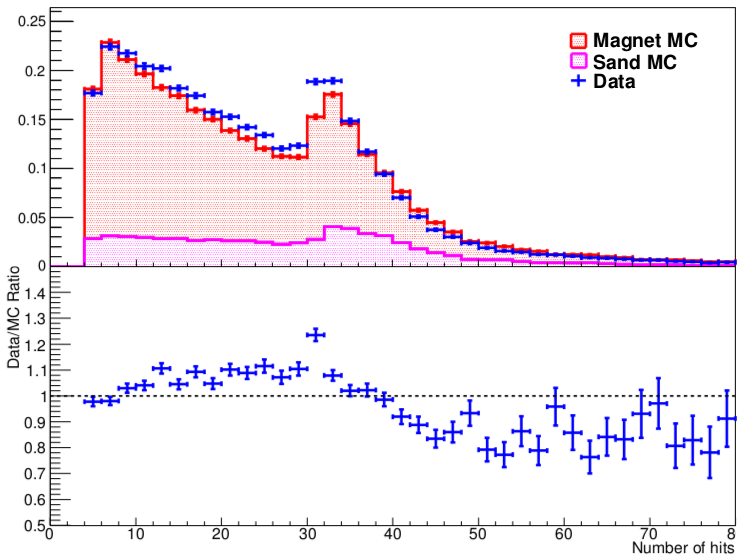
\includegraphics[width=9cm]{images/magnetic_field/NHits_BLB_NoField} \label{fig:NHitsBLBNoField}}
  \subfloat[The truncated max ratio of the reconstructed cluster.]{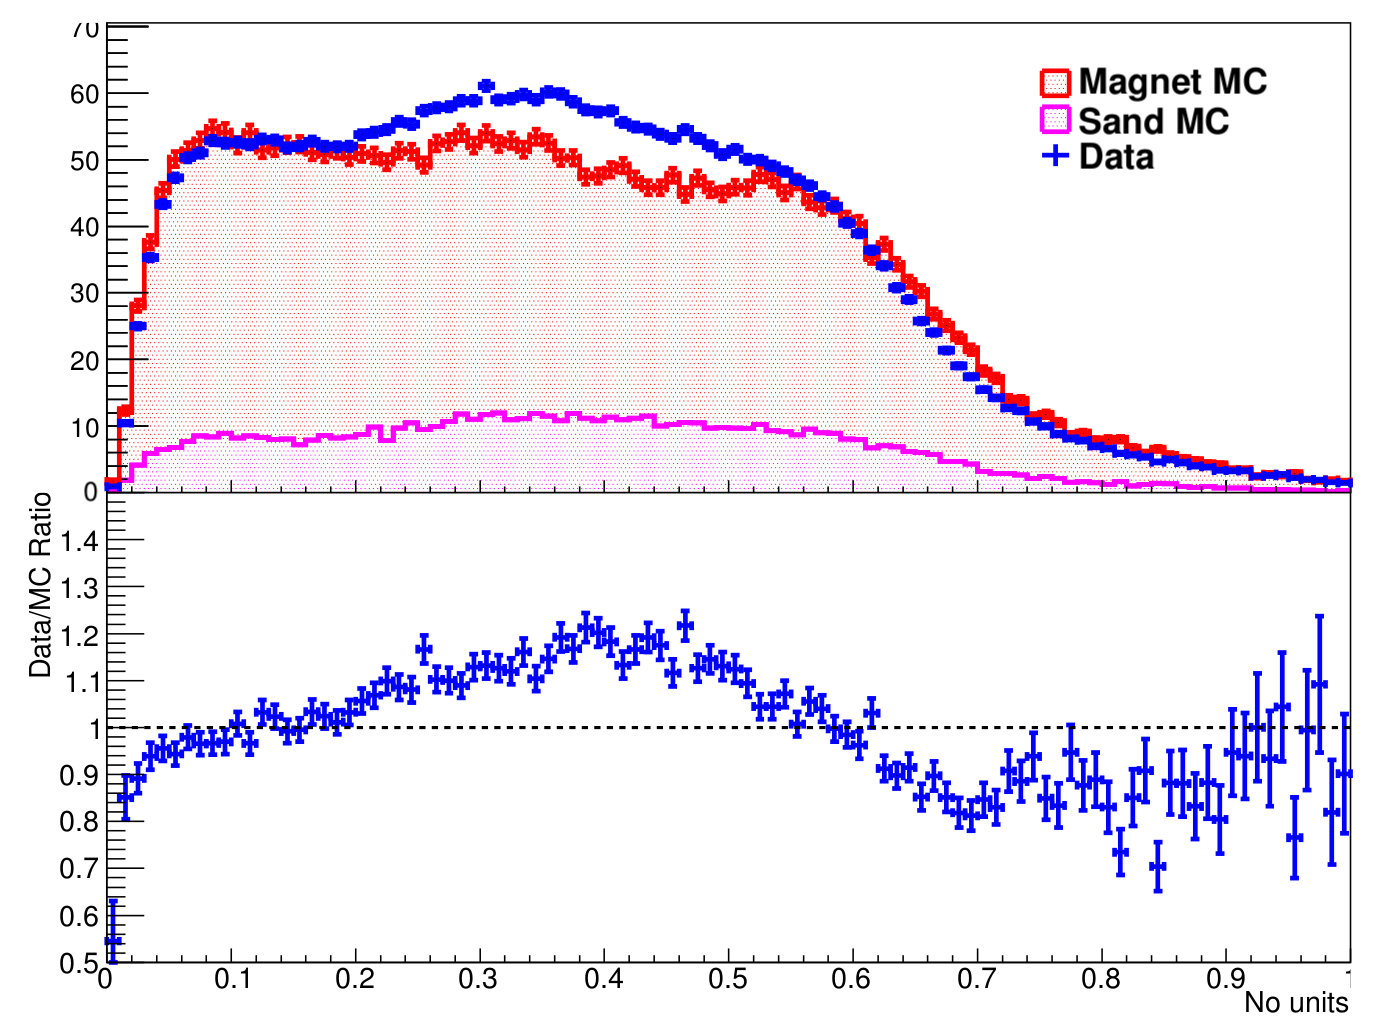
\includegraphics[width=8cm]{images/magnetic_field/TMR_BLB_NoField}\label{fig:TMRBLBNoField}}

  \caption{Comparisons of data and Monte Carlo in the bottom-left barrel ECal for previous software productions.  The red and pink histograms are Monte Carlo simulation of T2K beam neutrinos incident on ND280 and the surrounding pit respectively.  The blue data points are collected data from run 3C.  Both of the plots are POT normalized.}
  \label{fig:BLBNoField}
\end{figure}
It was found in previous iterations of ND280 analyses that there were significant discrepancies between the Monte Carlo and the collected data in the ECal.  The discrepancies found had an ECal module dependence where the bottom modules were affected most.  The problem appeared in the low-level distributions, such as how many scintillator hits were assigned to each reconstructed object.  An example of this is shown in Fig.~\ref{fig:NHitsBLBNoField} which shows a comparison of Monte Carlo with run 3C data for the number of constituent hits in each reconstructed object measured in the bottom-left barrel ECal.  For the number of hits region with high population (between roughly 10 and 30) there is a clear excess of collected data events.  As the high level variables, such as the ones used for track-shower discrimination, are based on these low-level quantities, the discrepancy propagated through causing significant disagreement at all levels.  An example of this effect is shown in Fig.~\ref{fig:TMRBLBNoField} which shows a data and Monte Carlo comparison, again for the bottom-left barrel ECal, for the Truncated Max Ratio (TMR) of the reconstructed objects.  The TMR, which calculates the ratio of the lowest total charge found in an ECal layer to the high total charge in an ECal layer after removing the top and bottom 20$\%$ of hits, is an input into the track-shower discriminator described in section~\ref{subsec:ECalParticleIdentification}.  The track-shower discrimination is a key feature of the ECal reconstruction which is used by several ND280 analyses so such a big discrepancy is a serious problem.
\newline
\newline
As ND280 is off-axis relative to the T2K beam, there is an increase in the neutrino flux in the flux return yoke and surrounding pit regions below the bottom ECals.  This means that any charged final states in this region would generally have to propagate through the flux return yoke.  If a magnetic field is present in this region, as there would be during data taking, the trajectory of such particles would be bent upwards towards the ND280 tracker region, causing an increase in the event rate in the bottom ECals.  If the magnetic field in this region is missing, the above statement does not hold and a relative deficit of events would be seen which describes the situation seen in Fig.~\ref{fig:BLBNoField}.
\begin{figure}[bottom]%
  \centering
  \subfloat[Number of hits in the reconstructed cluster.]{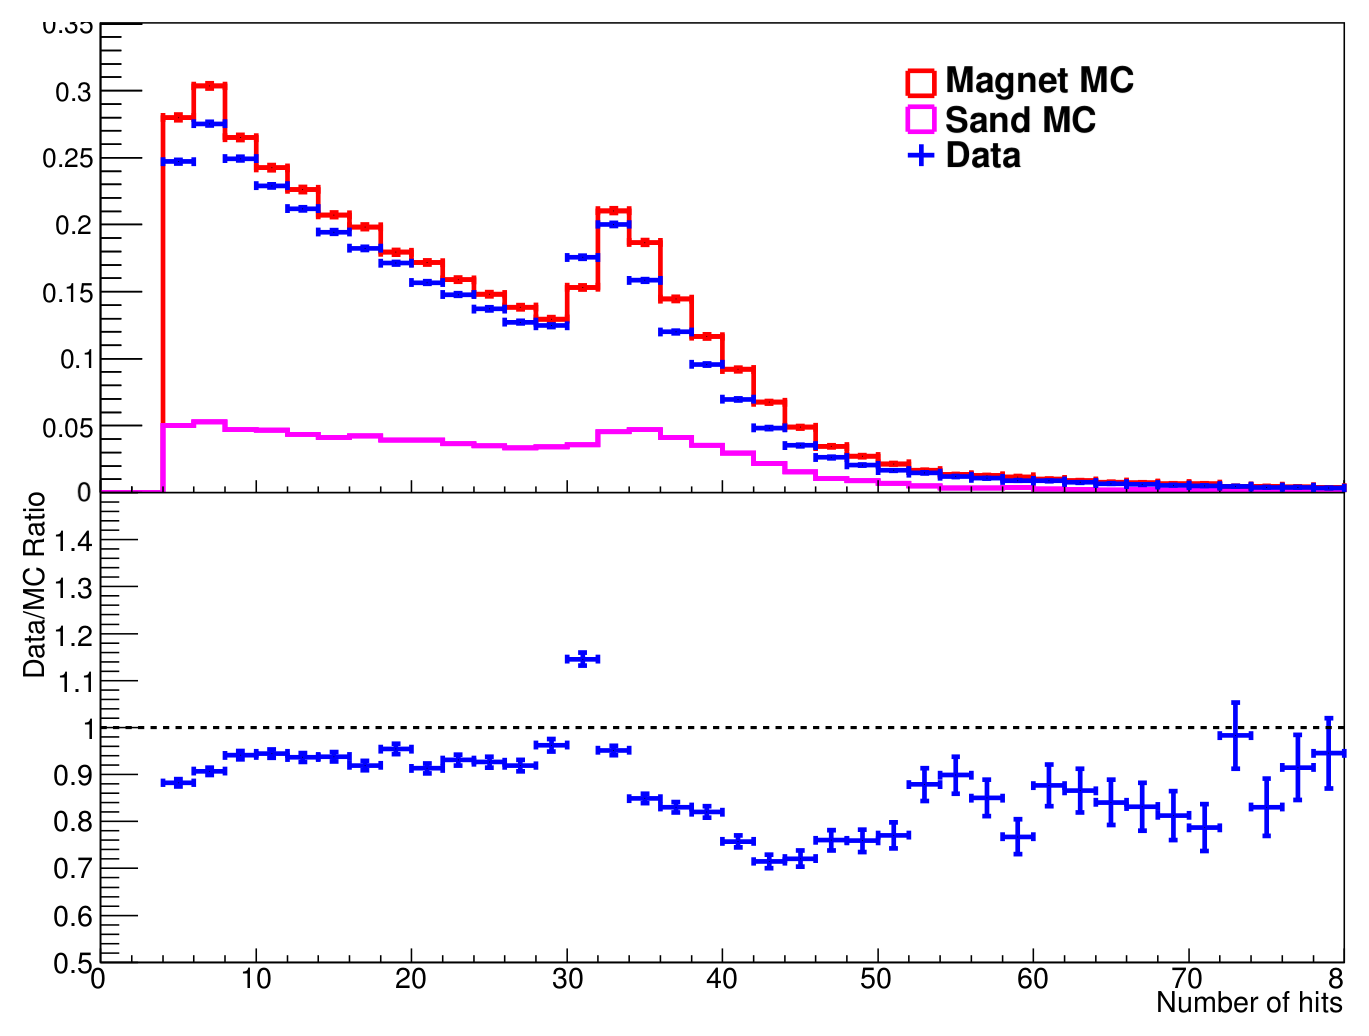
\includegraphics[width=8cm]{images/magnetic_field/NHits_BLB_WithField} \label{fig:NHitsBLBWithField}}
  \subfloat[The truncated max ratio of the reconstructed cluster.]{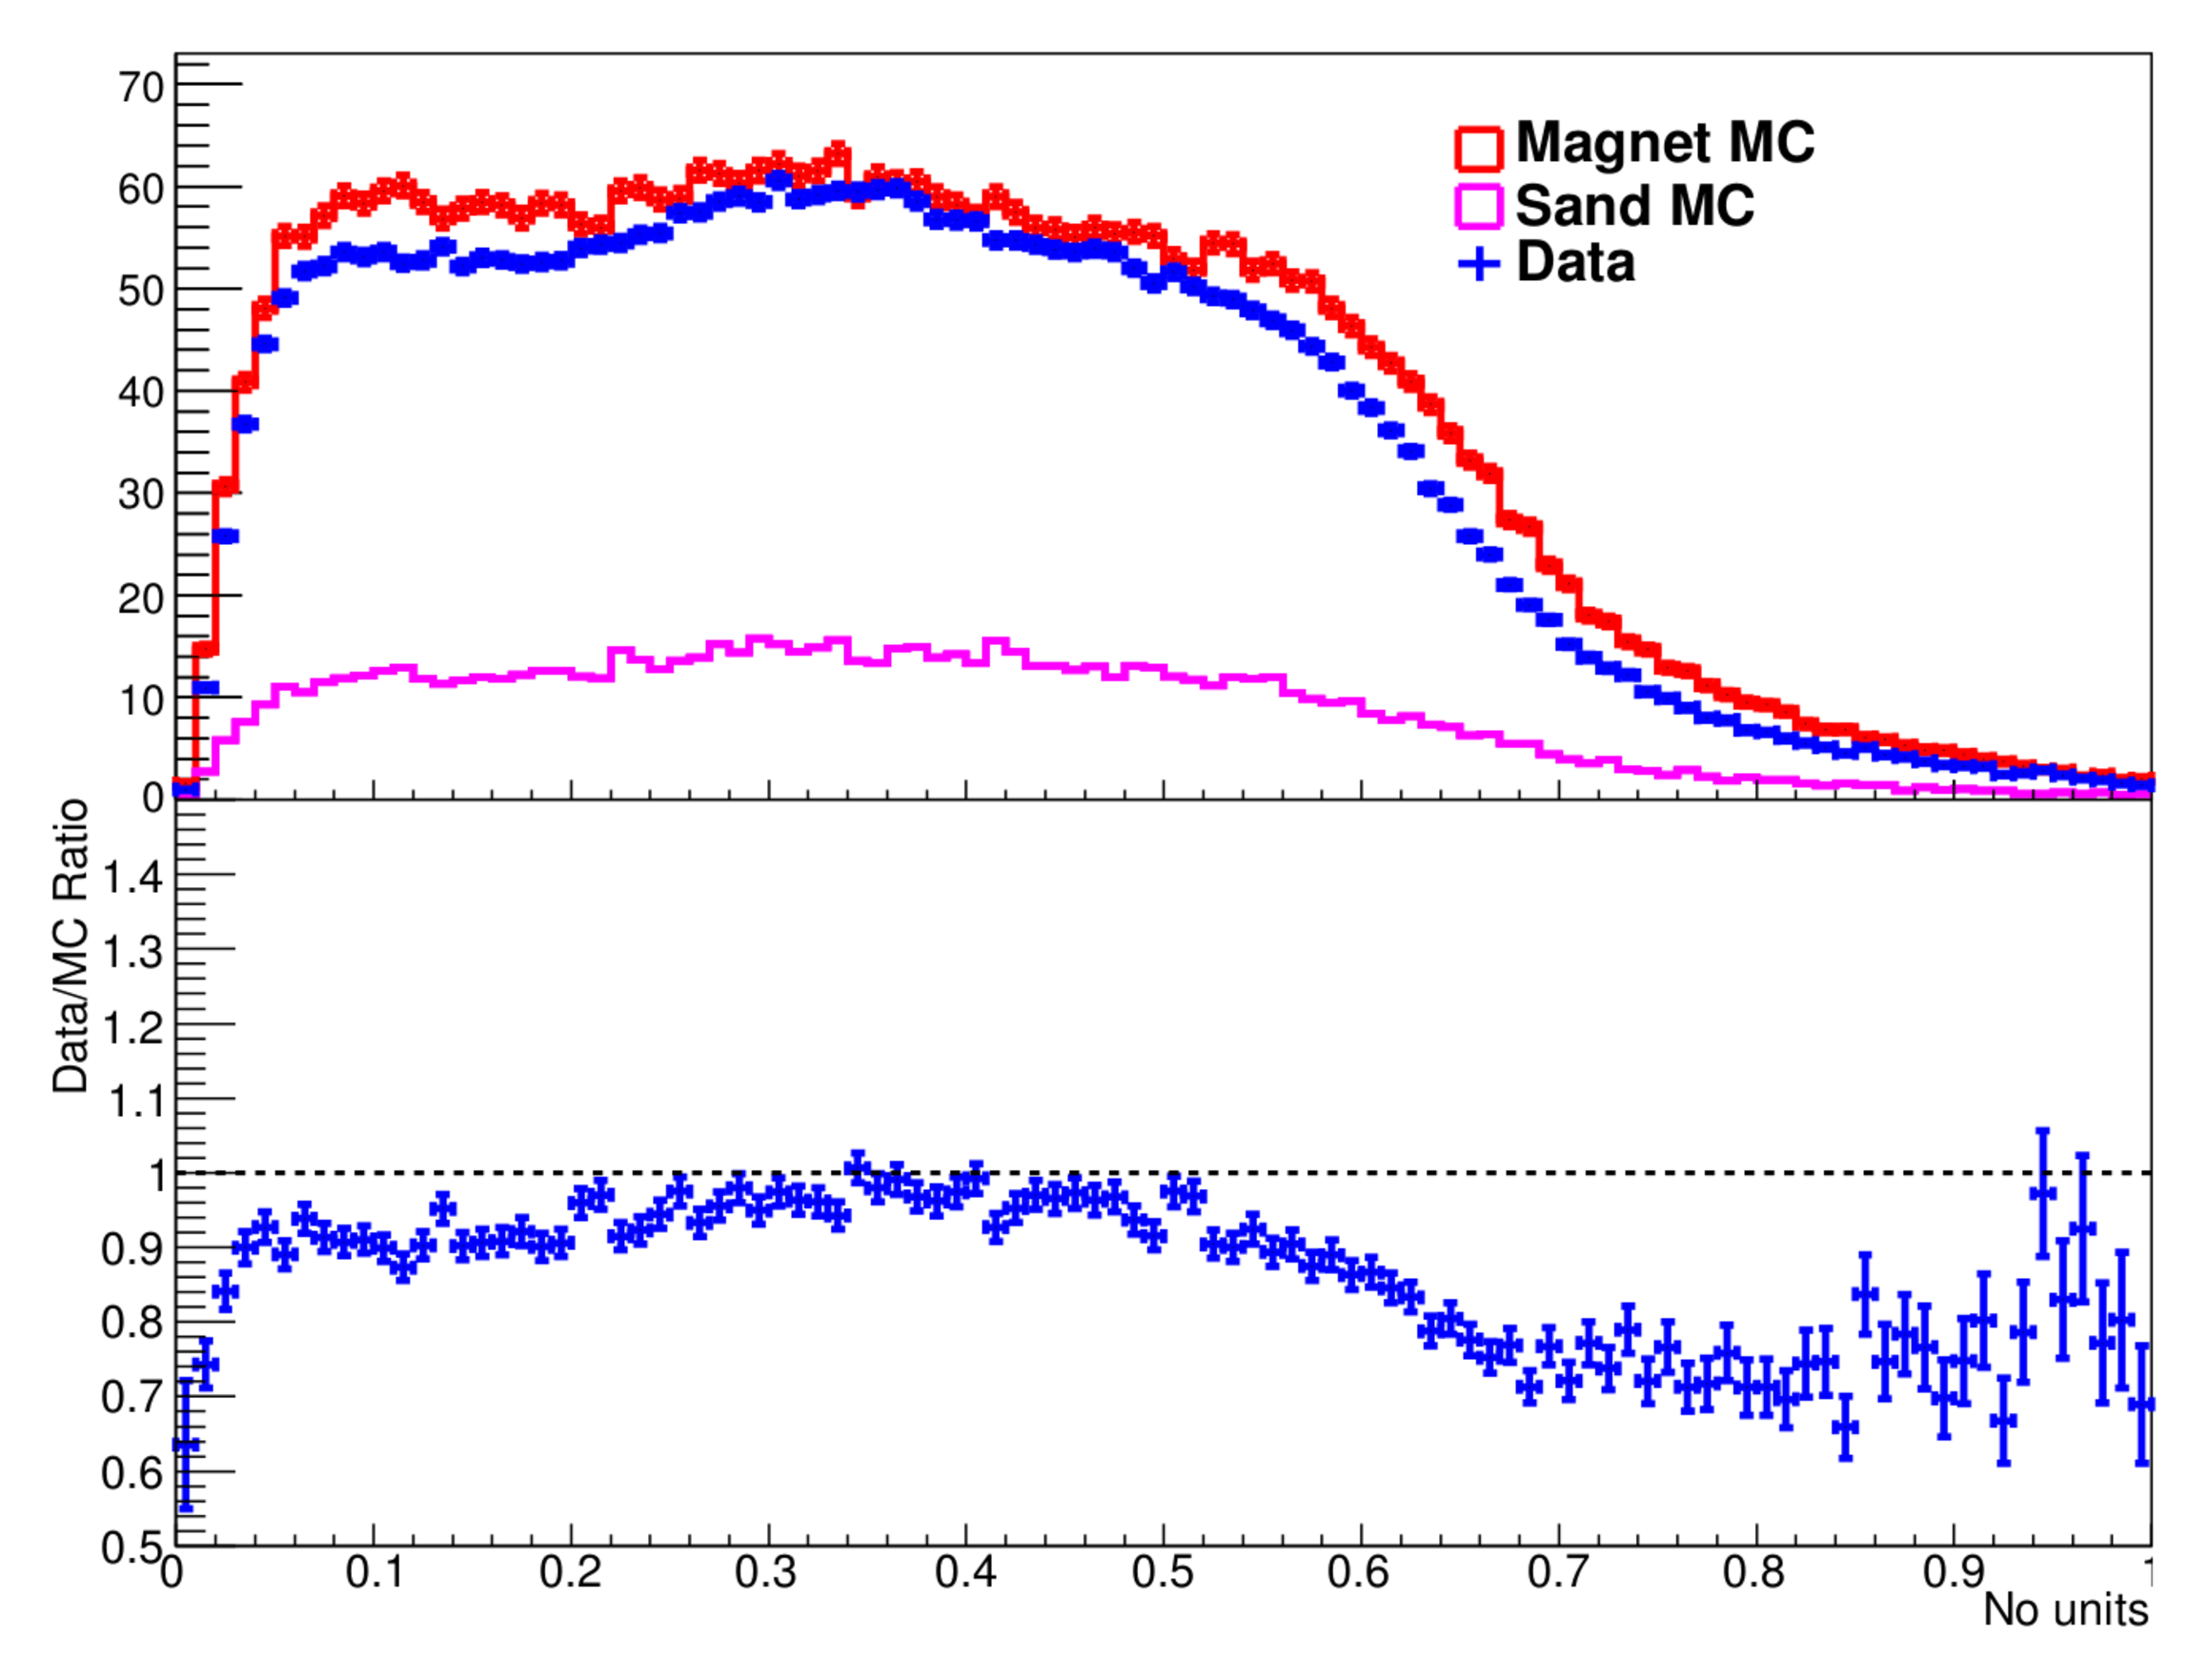
\includegraphics[width=8cm]{images/magnetic_field/TMR_BLB_WithField}\label{fig:TMRBLBWithField}}
  \caption{Comparisons of data and Monte Carlo in the bottom-left barrel ECal with the magnetic field model described in section~\ref{sec:MagneticFieldModel} implemented.  The red and pink histograms are Monte Carlo simulation of T2K beam neutrinos incident on ND280 and the surrounding pit respectively.  The blue data points are collected data from run 3C.  Both of the plots are POT normalized.}
  \label{fig:BLBWithField}
\end{figure}
So, the simple magnetic field model in the flux return yoke described in section~\ref{sec:MagneticFieldModel} was implemented in nd280mc and a batch of beam and \Yoshi{sand Monte Carlo}{``sand Monte Carlo'' is very much jargon. Introduce it properly} was produced to test its effect.  To get an idea of the magnetic field's effect on the rates measured by the ECals, the same variables as shown in Fig.~\ref{fig:BLBNoField} are shown in Fig.~\ref{fig:BLBWithField}, but with the magnetic field activated.  The difference is very clear; Fig.~\ref{fig:NHitsBLBWithField} shows that the excess in the 10 to 30 hits region is now gone.  It is also clear that the effect of the magnetic field has propagated through to the high level discriminators, as shown in Fig.~\ref{fig:TMRBLBWithField}.
\newline
\newline
Despite this study only briefly investigating the presence of a magnetic field in the UA1 flux return yoke, the improvement provided is undeniable.  It was decided that the model would be a permanent feature of the ND280 simulation and is now used in all software productions including the inputs to this analysis.
